%!TEX root = paper.tex

\section{Results}
\label{sec:bluetooth}

In this section, we present the results of our 19~month study of Bluetooth
devices observed with Bluetana at \visitedgasstations~gas stations across six U.S.
states (CA, AZ, NV, MD, IL, NC).
%
During the course of this study, Bluetana detected \totalskimmers~skimmers operating in \Bluetanaskimstations~gas
stations; all of the skimmers were removed from the pumps by local and
federal law enforcement agents.
%
Bluetooth scanning is a surprisingly effective way of detecting skimmers: in
Arizona, Bluetana has detected skimmers at 1.58\% of the \visitedgasstationsAZ~stations it
scanned, and routine inspections by state
inspectors had a similar detection rate of~\azpercentskimfound~from 2016 to 2018.
 
The primary result of this study is as follows: there are distinct characteristics of the
~\totalskimmers~internal skimmers detected by Bluetana that differentiate
them from the 2,562 other Bluetooth devices that Bluetana found 
at gas stations (e.g., car stereos).
%
Namely, these skimmers were predominately using the default Bluetooth module configuration.
%
Additionally, we discovered that some criminals use a custom Device Name 
in an apparent attempt to hide their skimmers from Bluetooth scans.
%
These custom Device Names stand out, making them easier to differentiate from other devices.

%Simply filtering by the~\visitedgasstations~gas stations to those that have devices matching two properties of skimmers---their
%Class of Device and their MAC prefix---leaves only \visitedstationsMACCoDfiltered~stations.

%, out of \visitedgasstations~gas.
%
\begin{comment}
Additionally, we discovered that the only technique that criminals use today to
do to hide skimmers in Bluetooth scans---using a custom Bluetooth device
name---actually makes it easier to differentiate the skimmers from other
devices. \noteby{MB}{We now know this not to be completely true...}
\end{comment}
%
\begin{comment}
surprisingly, one station was infected with skimmers twice during the
course of the study, and two skimmers were still installed six months after we initially detected them\footnote{These skimmers were discovered by looking back at our dataset after we discovered a new way that skimmers appear in Bluetooth scans.}.
\end{comment}
%
%Surprisingly, 81.3\% of
%these devices appear to be legitimate products that use the same Bluetooth
%modules that criminals use in skimmers (e.g., engine diagnostic monitors).


\subsection{What Do Skimmers Look Like in Scans?} %{{{
\label{sec:bluetooth:skimmers}

We begin by presenting how skimmers we observed appear in Bluetooth scans.
%
We describe the properties of two sets of skimmers: \totalskimmers~skimmers that we detected in the field
during the course of this study, as well as \totalskimmersLE~skimmers that were independently recovered by two LE agencies.
%
The \totalskimmersLE~skimmers recovered independently by LE have similar characteristics to the \totalskimmers~that Bluetana detected in the field.
%
%The default name often incorporates the product name or the name of the
%manufacturer, and part of the MAC address (e.g., RNBT-12AB'' for a Roving
%Networks Bluetooth serial module with MAC that ends in ``12AB'')
%
The Bluetooth characteristics of these skimmers are
detailed in Table~\ref{tab:skimmer-data-overview}.
%
We now analyze the following properties: Class-of-Device, MAC prefix, and Device Name. 
%In this analysis, we added an additional \totalskimmersLE~skimmers beyond the \totalskimmers~that
%Bluetana detected, and were provided to us directly by law enforcement.

\begin{table}[!h]
    \centering
    \captionsetup{justification=centering}
    \caption{Bluetooth scan properties of skimmers observed during our study.
    %
    The exact Device Names are not shown, instead we describe the names we found.
    }
    \begin{tabular}{lll}
    \toprule
    & \multicolumn{2}{c}{\colname{\# of skimmers}}\\
    \cmidrule(lr){2-3}
    \colname{Bluetooth Scan Property} & \colname{Bluetana}  & \colname{LE}\\
    \hline
    \textbf{Class-of-Device} \\
    \quad Uncategorized & 64 & 23 \\
    \hline
    \textbf{Manufacturer (MAC prefix)} \\
    \quad Roving Networks \\
    \quad \quad \texttt{00:06:66} & 45 & 13 \\
    \quad Shenzhen Bolutek \\
    \quad \quad \texttt{98:D3:31} & 1 &  \\
    \quad \textit{Unknown}  \\
    \quad \quad \texttt{20:13:04} & 1 &  \\
    \quad \quad \texttt{20:17:11} & 1 &  \\
    \quad \quad \texttt{20:18:01} & 2 &  \\
    \quad \quad \texttt{20:18:04} & 1 &  \\
    \quad \quad \texttt{20:18:07} & 1 &  \\
    \quad \quad \texttt{20:18:08} & 4 & 10 \\
%    \footnote{The HC-05 modules skimmers use have MAC addresses which
%    are configured at manufacturing time to match the date.}
    \quad \quad \texttt{20:18:09} & 4 &  \\
    \quad \quad \texttt{20:18:10} & 1 &  \\
    \quad \quad \texttt{20:18:11} & 2 &  \\
    \quad \quad \texttt{98:D3:35} & 1 &  \\
    \hline
    \textbf{Device Name} \\
    \quad \textit{Default} & 36 & 23\\
    \quad [Law enforcement] & 2 & \\
    \quad [Mobile phone] & 4 & \\
    \quad [Indescript object] & 2 & \\
    \quad [Numerical] & 2 & \\
    \quad \textit{Unnamed} & 18 & \\
    \midrule
    \midrule
    \textbf{Total} & 64 & 23 \\
    \bottomrule

\end{tabular}

\begin{comment}
\begin{tabular}{lll}
    \toprule
    & \multicolumn{2}{c}{\colname{\# of skimmers}}\\
    \cmidrule(lr){2-3}
    \colname{Bluetooth Scan Property} & \colname{Field}  & \colname{Officials}\\
    \hline
    \textbf{Class of Device} \\
    \quad Uncategorized & 37 & 23 \\
    \hline
    \textbf{Manufacturer (MAC prefix)} \\
    \quad Roving Networks \\
    \quad \quad \texttt{00:06:66} & 27 & 13 \\
    \quad Shenzhen Bolutek \\
    \quad \quad \texttt{98:D3:31} & 1 &  \\
    \quad \textit{Unknown}  \\
    \quad \quad \texttt{20:13:04} & 1 &  \\
    \quad \quad \texttt{20:17:11} & 1 &  \\
    \quad \quad \texttt{20:18:01} & 2 &  \\
    \quad \quad \texttt{20:18:08} & 3 & 10 \\
    \quad \quad \texttt{20:18:09} & 1 &  \\   
%    \footnote{The HC-05 modules skimmers use have MAC addresses which
%    are configured at manufacturing time to match the date.}
    \quad \quad \texttt{98:D3:35} & 1 &  \\
    \hline
    \textbf{Advertised Name} \\
    \quad \textit{Default} & 21 & 22\\
    \quad [Law enforcement] & 2 & \\
    \quad [Mobile phone] & 2 & \\
    \quad [Indescript object] & 1 & \\
    \quad [Numerical] & 2 & \\
    \quad \textit{Unnamed} & 9 & 1\\
    \midrule
    \midrule
    \textbf{Total} & 37 & 23 \\
    \bottomrule

\end{tabular}
\end{comment}


    \label{tab:skimmer-data-overview}
\end{table}

\subsubsection*{All of the skimmers are ``Uncategorized'' Class-of-Device}

Class-of-Device 
%
is primarily 
used to select the icon that indicates the category of a device in a Bluetooth
scan (e.g., Headphones).
%
Bluetooth modules used in skimmers analyzed in this study (i.e., HC and RN), have an ``Uncategorized''
Class-of-Device assigned by default. 
%The factory default Class-of-Device for the Bluetooth modules used in the
%skimmers we analyze in this study (i.e., HC and RN) is ``Uncategorized''.
%
Changing Class-of-Device on these modules is trivial: the modules provide a serial
command to set it.
%
Despite this, criminals do not appear to be modifying the Class-of-Device on
any of the skimmers we observed:
%
all of the \totalskimmersseen~skimmers detected by Bluetana and recovered independently by LE
used the default ``Uncategorized'' device class.
%
%Class-of-Device is not considered by existing Bluetooth-based skimmer
%scanning applications available on the Play Store~\cite{scaifeoakland}.

\subsubsection*{MAC prefixes are often manufacturer defaults}



Bluetooth module manufacturers burn a MAC address into the module's EEPROM.
%
Although it is possible to change the MAC with a SPI-based
reprogramming of the CSR chip's EEPROM, we have not observed any skimmers that have a modified MAC.
%
The first three bytes (prefix) of the MAC address typically correspond to the
manufacturer of the device. 
%
%Several applications use this
%as the primary way of detecting skimmers~\cite{scaifeoakland}.


Although MAC address prefixes are often assigned by IEEE (e.g., all of the RN Bluetooth modules have the same manufacturer MAC prefix) the HC modules have a wide
%
variety of MAC prefixes.
%
Of the HC modules we observed, only one has a MAC prefix assigned by the IEEE.
% 
This could make it significantly more difficult to detect an HC-equipped
skimmer.
%
However, looking at of the MAC prefixes of the skimmers that we observed, a clear pattern
emerges: manufacturers appear to be burning module manufacture date into
the first four bytes of the MAC address in the following format:
\texttt{YY:YY:MM:(DD)}.
%
%Section~\ref{sec:ops:macs} we show that we can use manufacturer MAC
%assignment patterns like these to several Bluetooth modules with
%similar MAC address may be from the same crew \noteby{JC}{address possibly originated from the same crew}.


\subsubsection*{Device names are often default, occasionally customized}

Device Names allow users to identify their devices in Bluetooth scans.
%
They are assigned a factory default value by the manufacturers, and are modifiable by users.
%
%allowing users to .
%
Most of the skimmers we observed had a default Device Name: namely, all of the skimmers provided by LE, and more than half the skimmers we detected in with Bluetana. 
%
%We observed that criminals did not change the factory default name that module
%manufacturers had assigned across all skimmers analyzed in the lab, and more
%than half of the skimmers we detected in the wild \noteby{JC}{}.
%
A skimmer with a default Device Name looks innocuous, because some legitimate products using the same modules are also shipped with the default module name (Section~\ref{sec:falsepositive}).
% 
Occasionally, we found that criminals set a custom device name on their skimmers.
%
This appears to be an attempt to make the skimmer look less suspicious.
%
Bluetana detected custom-named skimmers with a variety of names. 
%
The custom names of skimmers discovered by Bluetana had variety: some were random strings of numbers, and others masqueraded as LE.
%
%, custom names have an opposite effect to what the criminals intended: they
%make it easier to detect these devices as skimmers, because is uncommon to see
%a Bluetooth module with a customized Device Name \noteby{JC}{because it is
%uncommon to see a commodity Bluetooth module with a customized Device
%Name~\footnote{Customized device names excludes known product names that use
%RN or HC modules}}
 
Bluetana did not detect a Device Name for several skimmers.
%
This is expected because the device sends its MAC and Class-of-Device in the first scan response packet; it sends the device name in a subsequent packet (that may be missed).

%Device Name packets may not be received properly:
%
%a device announces its Device Name in a second packet following the first packet that contains the MAC and Class-of-Device.

%The name comes in the next part of the scanning process where the scanner sends
%a remote name request, and the skimmer responds with its name.
%
%The process is as follows, the master device will send an inquiry packet on a
%variety of frequencies, and it will wait for a response from the skimmer.

\subsubsection*{Skimmers are detected within one minute}

\begin{figure}
\centering
\captionsetup{justification=centering}
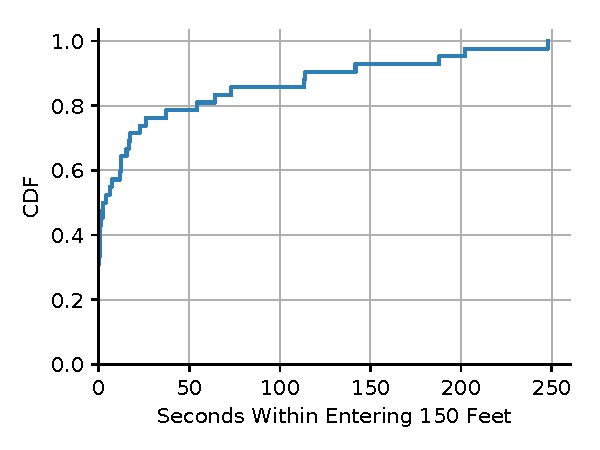
\includegraphics[width=0.6\linewidth]{skimmer/plots/cdf_skim_discover_time.pdf}
\caption{
\label{fig:skim_discover_time}
 Skimmers are detected within a minute of passing near a gas station.
}
\end{figure}

Bluetooth scanning has the benefit of detecting some skimmers without manually inspecting each of the pumps.
%
However, attenuation from a gas pump's metal enclosure, may limit the range that Bluetooth scans are effective.
%
We analyzed the scans from Bluetana to see how long an official had to spend at a gas station before they detected the skimmers installed there (Figure~\ref{fig:skim_discover_time}).
%
%time instant when the officials driving within 150 feet of gas station first
%detected the skimmers that were there
%
The median time to detection was \skimmerdetectiontimemedian~seconds, and \skimmeroneminutepercent~of the skimmers were detected within one minute.
%
This is a 99\% decrease in search time compared to the average of 30 minutes
that inspectors take to check a gas station for skimmers.\footnote{Source:
discussions with inspectors.},
%
This result indicates that inspectors can quickly stop at gas stations to check for Bluetooth-detectable internal skimmers.

%Officials detect skimmers take an average of 30 minutes to inspect all of the pumps at a gas
%station to detect if a skimmer is present.
%
%Also, Bluetooth scans can take up to 20~seconds to complete.
%


%}}}

\subsection{Are Skimmers Distinguishable in Scans?} %{{{
\label{sec:bluetooth:scans}

\begin{table}
    \centering
    \captionsetup{justification=centering}
    \caption{On average there are two Classic Bluetooth devices seen at each gas
    station; infrequently, there are skimmers.
    }
    \begin{tabular}{llllllr}
    \toprule
    &  & \multicolumn{3}{c}{\colname{Devices Observed}} \\
    \cmidrule(lr){3-5}
    \colname{State} & \colname{Stations} & \colname{\#} & \colname{Avg.} & \colname{Std.} & \colname{Days} & \colname{Skimmers}\\
    \midrule
    CA & 571 & 1148 & 2.01 & 1.94 & 152 & 22 \\
    AZ & \visitedgasstationsAZ & 1140 & 2.32 & 2.03 & 130 & 36 \\
    NV & 38 & 93 & 2.45 & 3.44 & 21 & 4 \\
    MD & 23 & 42 & 1.83 & 1.86 & 14 & 2 \\
    IL & 18 & 37 & 2.06 & 2.01 & 13 & 0 \\
    NC & 10 & 20 & 2 & 1.67 & 10 & 0 \\
    \bottomrule
\end{tabular}


    \label{tab:data-overview}
\end{table}





Next, we evaluate if 
the skimmers detected by Bluetana were clearly distinguishable from the other devices observed at gas stations. 
%
%We collected these Bluetooth scans from~\visitedgasstations~gas stations across
%six states, giving us a comprehensive view of what Bluetooth
%devices tend to appear at a typical gas station in these states.
% 
The primary result of this study is that these skimmers were not
hidden well.
%
Many of these skimmers use the default configuration of their Bluetooth
modules.
%
Legitimate devices using the same Bluetooth modules may have some default parameters, and a few have all of parameters set to the default.
%
We conclude that by combining multiple characteristics: MAC prefix, Class-of-Device,
and Device Name, there are only a small number of devices that could be
confused with skimmers.

This study also reveals that when criminals creatively modify their skimmer's
Device Name, it makes detection easier.
%
We also found that criminals could improve how they hide skimmers in Bluetooth
scans.
%
For example, they could change the Class-of-Device to hide as a more popular
device (e.g., a smartphone).

\subsubsection*{Dataset Overview} %{{{

Over the course of the 19~month study, Bluetana users visited ~\visitedgasstations~ gas
stations across six states (Table~\ref{tab:data-overview}).
%
During these visits, Bluetana detected a total of~\totalskimmers~skimmers---all of which were recovered by officials.
%
These skimmers were in the presence of ~\totalbtobserved~ other devices.
% 
On average, Bluetana saw \averageclassicBTperstation~devices per
station ($\sigma = \stdevclassicBTperstation$).
%
Given that there are only a small number of Bluetooth devices seen per station,
it may seem likely that these devices are all skimmers.
%
However, only a small fraction (\pctmatchskimmer) of these devices matched the
characteristics of the skimmers we observed during the course of our study. 
%
%In fact, Bluetana only detected skimmers at \Bluetanaskimstations~gas stations out of the.

%In , we provide a summary of the number of skimmers and 
%Bluetooth devices that we observed during the study.
%
We performed this study on Classic Bluetooth devices only.
%
We did not include BLE because we are not
aware of any internal gas station skimmers using BLE modules.
%
However, we observed a large number of BLE devices at gas stations; therefore, switching skimmers to
BLE modules may make them more difficult to detect with
scanning tools like Bluetana (Section~\ref{sec:hiding:ble}).


%\subsubsection*{Restricting scans to those that occur at gas stations}
%
%Bluetana scans constantly, it may detect devices that are outside of gas
%stations.
%
For this analysis, we only include the scan data that is collected the first
time a Bluetana user visits a station.
%
Restricting the dataset in this way ensures fairness in our results. Analyzing all
inspections may bias our observation of what Bluetooth devices tend to be found at gas stations to those that
were visited multiple times.
%
Specifically, we only analyze scans
performed the first time Bluetana is near a gas station (within 150 feet) for
at least 30 seconds and up to 5 minutes.
%
22 out of 64 of the skimmers were detected on subsequent
visits to gas stations, so they are not included in this analysis.
% 
%This distance is the equivalent of approximately 10 mid-sized
%sedans~\cite{us40cfr600}.
%
%\todo{In California, where they do not do routine inspections, the 22 skimmers
%were all not seen at all before.}

%}}}

\begin{figure}[!h]
    \centering
    \captionsetup{justification=centering}
    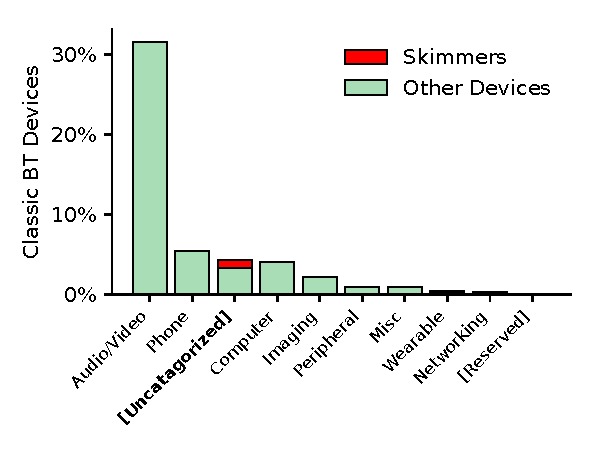
\includegraphics[width=0.6\linewidth]{skimmer/plots/hist_device_class.pdf}
    \caption{
    \label{fig:hist_device_class}
    Skimmers appear in the third most common class of Bluetooth devices.
    }
\end{figure}
\subsubsection*{Skimmers are Uncategorized, but so are other devices} %{{{

The only Bluetooth property that is common among all skimmers we observed is
that they have an Uncategorized Class-of-Device.
%
Figure~\ref{fig:hist_device_class} shows the distribution of Bluetooth device classes at gas stations.
%
Uncategorized devices are the third most common Class-of-Device found by Bluetana (\percentbtuncategorized~of devices).
%
Although, out of the \visitedgasstations~gas stations that Bluetana users visited, Uncategorized devices were only observed at \totaluncatstation~gas stations (12.1\%).
%}}}




\subsubsection*{Other devices use the same modules as skimmers} %{{{

%\begin{figure}
%\centering
%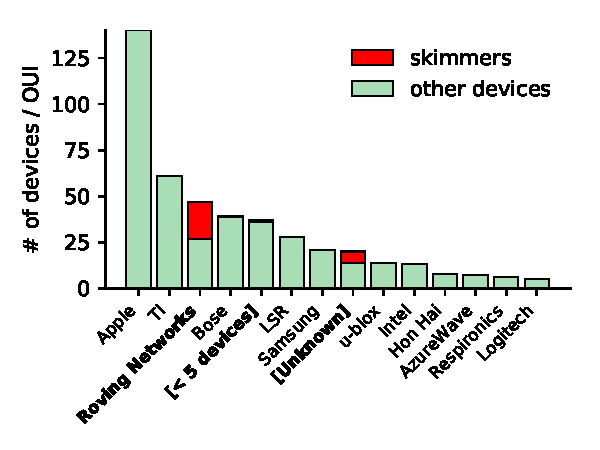
\includegraphics[width=\linewidth]{plots/all_hist_device_OUI.pdf}
%\caption{
%\label{fig:hist_device_OUI}
%Distribution of manufacturers per gas station visit. Skimmers are common amongst Roving Networks and unassigned
%manufacturers, and also occasionally smaller module producers.
%}
%\end{figure}



Within the set of Uncategorized devices, we next look at the distribution of
their MAC prefixes (Figure~\ref{fig:hist_device_OUI}).
%
 %shows the distribution of Unclassified device AC prefixes observed by
%Bluetana at gas stations (listed by manufacturer).
%
We find that the Bluetooth modules used in skimmers are also used in many other legitimate
devices.
%
Specifically, more than half of the RN modules seen at gas stations were in
skimmers, but there were many other devices that had RN modules.
%
%It is possible to identify many skimmers by looking at the MAC address of the
%discovered device and checking it against a hit-list of known skimmer module
%manufacturers.
%
%This hit-list is sourced from reports from law enforcement and previously
%discovered skimmers
%
This is an important observation because a popular detection application,
SkimPlus~\cite{skimplus}, only flags skimmers based on a hitlist of MAC
prefixes~\cite{scaifeoakland}; it may incorrectly flag legitimate devices as
skimmers.

\begin{figure}[!h]
    \centering
    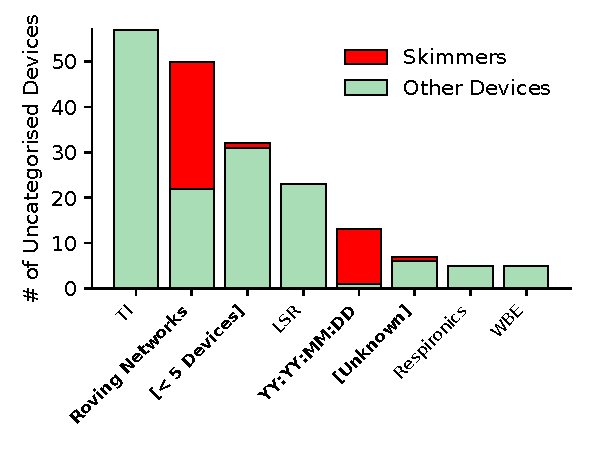
\includegraphics[width=0.6\linewidth]{skimmer/plots/uncat_hist_device_OUI.pdf}
    \caption{
    \label{fig:hist_device_OUI}
    Many other devices appear to be using the same Bluetooth modules as skimmers.
    }
\end{figure}

The devices observed with MAC prefixes that were in the \texttt{YY:YY:MM:DD}
format (likely HC modules) were mostly skimmers.
%
There were many devices that had IEEE assigned MAC prefixes that were
infrequently seen at gas stations ($<5$ Devices). Only one of these devices
was a skimmer.
%
Also, there were many devices with MAC prefixes unknown to the IEEE, but not in
the date format, only one of these devices was a skimmer.
%
Overall, \numberBTMACCoDfiltered~devices out of
\numberbtuncategorized~Uncategorized devices matched the MAC prefixes of
Bluetana-observed skimmers.
%Of the devices that had the same MAC prefix as observed skimmers, only
%\numberBTMACCoDfiltered~devices matched these MAC prefixes (out of
%\numberbtuncategorized~Uncategorized devices).
%
This reduces the number of stations where Bluetana detected skimmers to
\visitedstationsMACCoDfiltered~out of the~\totaluncatstation~stations where it found
Uncategorized devices.



%
%It was discovered that this MAC address was questionable after another HC-05
%module close in MAC range had been discovered by investigators.
%
%The device also had a distinctive name which allowed it to be flagged
%independently of OUI.
%
%There were also other devices with MAC prefixes not matching known IEEE assignments, that were not skimmers.
%
%For one of these skimmers, it was clear that the MAC was either purposefully
%misconfigured by the criminal or by the manufacturer of the module.
%
%For all HC-05 modules but two, the MAC addresses were simply the date of
%manufacture in the YY:YY:MM:DD format mentioned earlier.

\if 0 %what is this?
Collaborating with law
enforcement, we were able to develop a hit-list consisting of X addresses. In
fat, there was a case under which we found new manufacturers of skimmers, and
were able to use this new information to isolate skimmers we had seen 7 months
prior. The most common devices that we saw which were of the uncategorized
device class actually ended up being phones; we did not find any skimmers
masquerading as phones. We did see devices with no registered manufacturer. Some
of these were simply odd devices, others were skimmers.
\fi
%}}}
\begin{figure}[!h]
    \centering
    \captionsetup{justification=centering}
    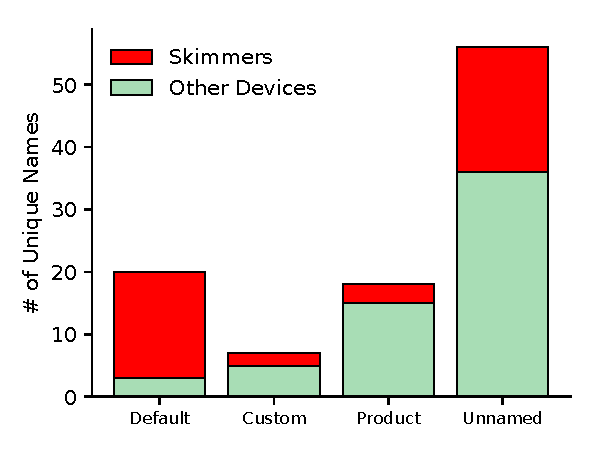
\includegraphics[width=0.6\linewidth]{skimmer/plots/uncat_visit_hist_device_name.pdf}
    \caption{
    \label{fig:hist_device_name}
    Default and custom names distinguish skimmers from legitimate devices.
    }
\end{figure}


\subsubsection*{Default- and custom-named modules are often skimmers} %{{{

Finally, we investigate if skimmers can be differentiated from other devices by
their Device Name.
%
The remaining~\numberBTMACCoDfiltered~devices are Uncategorized and their MAC prefixes are either: Roving Networks, \texttt{YY:YY:MM:DD}, Unknown, or seen on less than five devices.
%
Only
\totalskimmersfirstvisit~of these devices were confirmed to be
skimmers.\footnote{We do not include 22 of the Bluetana-detected skimmers in
this analysis because they were not detected on the first visit to a gas
station.}
%
In Figure~\ref{fig:hist_device_name}, we divide the remaining devices by their
category of Device Name, including: \emph{unnamed}, manufacturer
\emph{default}, known legitimate \emph{product}, and \emph{customized}.
%
Devices observed by Bluetana with default names were often skimmers.
%
Custom named devices were not common at gas stations but had a higher
probability of being skimmers.
%
Three skimmers were disguised as products, however all three were
distinguishable because their names were popular smartphones, which should not
have the MAC prefix of Bluetooth-to-Serial modules.
%
Bluetana missed capturing the Device Name for many of the skimmers, as well as other
devices that it detected.
%
 
%The relative portion of skimmers each category of  are 22.4\% for Unnamed,
%85.7\% for default, 6.9\% for product, and 33.3\% for custom.
%





%

%We have seen skimmers disguise their names as cell phones in 3 of our 37 detection cases, and as generic non-malicious
%entities in 4 other cases.
%
%However, as the criminals are not also modifying the OUI of the devices to match, this can actually be used as a clear
%flag that a given device is a skimmer, i.e. seeing a roving networks module advertising itself as a Bluetooth speaker.

%\subsubsection*{Summary}

%In summary, we 

%\todo{We are likely not missing skimmers}

%}}}

%}}}

\subsection{Accuracy of Bluetooth-based Detection} %{{{

To evaluate the accuracy of Bluetooth-based detection, we analyze Bluetana scan
data collected during inspections in Arizona. Specifically, there was a 7-month
time period in which Bluetana was used by many of the Arizona inspectors
(October 7, 2018 -- May 7, 2019), and we compare the reports filed during these
inspections with the scan data that Bluetana collected.

\subsubsection*{Missed skimmers}
\label{sec:falsenegative}

%o measure the accuracy of Bluetooth 

During this time period, there were 27 inspections where
skimmers were found while an inspector was running Bluetana.
%
A total of 42 skimmers were
recovered during these inspections, of which Bluetana was able to detect 36.
%
Therefore, Bluetana missed detecting 14.3\% of the total skimmers recovered during these inspections.

We do not know exactly why Bluetooth-based scanning missed these skimmers.
%
Half of the missed skimmers were from inspections where Bluetana detected other
skimmers at the gas station.
%
It is likely that these missed skimmers were not powered on due to
improper installation.
%
The remaining missing skimmers may have been built with alternate
exfiltration methods, such as SMS~\cite{scaifeoakland}, or even require physical
recovery~\cite{skimreaper2018}.

%Unfortunately, we were unable to test these skimmers in our lab because they
%were sent out to law enforcement immediately for further investigation.
%
	

\subsubsection*{Incorrectly detected skimmers}
\label{sec:falsepositive}

Bluetana highlighted a device in red during 45 Arizona inspections where no
skimmer was found.
%
There were 757 total inspections where inspectors used
Bluetana\footnote{This includes both routine and complaint/prior knowledge
triggered inspections},  Bluetana may have incorrectly detect skimmers in 5.9\%
of inspections.

%Considering Bluetana uses at least MAC prefix and Class-of-Device for
%highlighting, it is likely that these incorrectly classified 

Incorrectly identifying skimmers is likely due to the fact that  RN and HC
modules are used in a variety of legitimate products, some of which are seen in
and around gas stations.
%
We found RN and HC modules in radar-based speed limit signs, weather
sensors~\cite{rnbtweathersensor} automotive diagnostic scanners,
scales~\cite{rnbtscale} and fleet tracking systems~\cite{rnbteletrac}.
%
Some of these devices have Device Names that clearly indicate what product they
are, but would be confused with skimmers if the Device Name
is missing.
%
Unfortunately, several of these products also use the default Device Names on
their Bluetooth modules (\emph{RNBT-xxxx} or \emph{HC-05}).
%
These legitimate devices will look exactly like skimmers.
%
In such cases, inspectors will need to rely on RSSI localization to determine if these devices
are located inside a gas pump.
%}}}

\if 0 % extra text{{{
\subsection{Skimmer Detection Likelihood}
This analysis shows skimmers constitute X number of the visited gas station.

Names:

custom - this many stations (\%)
default - this many stations (\%)
unnamed - this many stations (\%)

The extent to which this characterization will hold true in the coming years, or the extent to which criminals are
developing mechanisms to ``mask'' the fingerprint of their devices is unknown.
%
We include an extended discussion of these factors in section~\ref{sec:discussion}.

Bluetooth detection has additional benefits.
%
In most of the cases in which our application detected anomalous devices, it was able to alert inspectors to skimmers
in pumps which they were not planning upon opening and inspecting.
%
This includes two cases under which the inspectors were simply ``driving by'' a gas station.
%
For five of the skimmers well hidden inside of their pumps, our application was able to determine with confidence
that a skimmer was in the pump despite an initial failed visual inspection.



Additionally, the following discussion does not use Bluetooth Low Energy (BLE) or SDP fingerprinting as detection
mechanisms.
%
BLE introduces complications to potential skimmer discovery which are outside of the scope of this paper.
%
While BLE skimmers have been found in countries outside of the United States, law enforcement in the six states we have
surveyed have not yet come in contact with a device using the protocol.
%
For more details, see section\ref{sec:ble}.
%
Similarly, SDP introduces complications and additional hardware costs which are addressed in section\ref{sec:SDP}.


%\begin{center}
%    \begin{tabular}{r|c|c|c}
%        \textbf{Module} & \textbf{Vendor} & Chip-set & \textbf{Range} \\ \hline
%        RN-\{41/42\} & Roving Networks & CSR 417 & 100m/30m \\ HC-\{05/06\} &
%        \textit{Various} & CSR 417 & 30m \\
%    \end{tabular}
%\end{center}
%
%
%Both modules reported several factory-default fields that uniquely identify
%them, specifically their manufacturer (MAC prefix known as IEEE OID) is a valid
%OID for the manufacturer (Roving Networks). For the HC device which is
%inexpensive, a squatted MAC OID that has not yet been assigned to a manufacturer
%by IEEE. Also, the modules have default Bluetooth names that indicate which
%module they are, and a default device class (i.e., None)---most products have a
%name and device class that reflects the product (e.g., name: ``Bose
%Quiet-Comfort'', class: ``Headphones'').
%%
%Criminals may stick with the default configuration, even though every one of
%these fields can be changed with some hacking (see
%Section~\ref{sec:discussion:hiding}) values because it makes something look
%innocuous.
%
%In summary, the Bluetooth modules commonly found in skimmers may be identifiable
%in Bluetooth scans.
%%
%However, all of the parameters are configurable, and to confirm this hypothesis
%we will need to study skimmers in the wild.
%%
%Designing an Android app to collect this will allow us to study a large number
%of gas stations and collect data on the Bluetooth environment.
%%
%This crowd sourced deployment will allow us to determine if skimmers can be
%reliably detected with Bluetooth inquiry scanning alone.



%\section{Implementation and Overview of Findings}
%
%
%
%To conclude this section, we will give an overview of the effectiveness of
%finding skimmers using the information above.
%
%From the recorded inquiry response data of 115,199 devices and 29,818 unique
%devices near gas stations, we were able to isolate \todo{X} skimmers.
%%
%The primary method used to isolate questionable devices was MAC address
%filtering based upon OUI.
%%
%This method paired with geo-location filtering alone is able to reduce the number
%of potential devices down to 677, at the cost of a potentially high
%false-negative and false-positive rate.
%%
%Not only did this method fail to find two skimmers who OUI's were not in the
%``hit-list'' initially \noteby{MB}{and maybe even more!}, it also flagged a lot
%of non-skimmers which were found to be above suspicion after a manual analysis
%of the other features listed above.

%The prior overview demonstrates the efficacy of combining multiple pieces of scan
%data when finding skimmers.
%%
%In the rest of the paper, we will examine our dataset and discuss the individual
%benefits and drawbacks of each feature listed above.
%%
%From this, we will develop an understanding of how the components work together
%and filter out the noise of the typical gas station environment and detect
%skimmers.

%\todo{NOW THE BELOW IS A SECTION}
%\begin{figure}
%    \centering
%    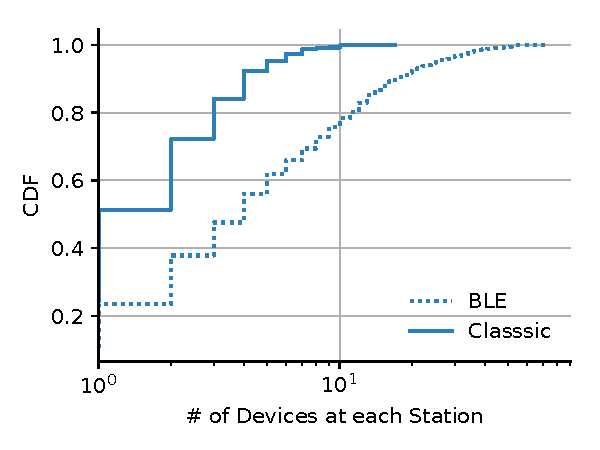
\includegraphics[width=\linewidth]{plots/cdf_num_devices_seen.pdf}
%    \caption{
%    \label{fig:cdf_num_devices_seen}
%    Distribution of the number of classic and low energy Bluetooth devices seen
%    in a visit to a gas station. Classic devices are far less common than
%    low energy devices.
%    }
%\end{figure}

%We are focusing this discussion only on devices that are Classic Bluetooth,
%because all modules used by recovered skimmers are classic Bluetooth.
%%
%In Section~\ref{sec:ble}, we will describe how Bluetooth Low Energy-based
%skimmers will complicate detection via Bluetooth Scanning.

%\subsection{Collection and Hunt Summary}

%

%\subsection{The Anatomy of a Skimmer Fingerprint}
%
%In this section we will concretize skimmer anatomy based upon those database records which we have confirmed to be
%skimmers and the criminal evidence to which we were given physical access.
%%
%
%Foremost, our understanding of Skimmer anatomy revealed itself in two stages.
%%
%During the initial phase of research, we manually examined each record of our dataset, with a goal of finding the
%offending devices directly.
%%
%Over time, this methodology was refined and automated, and a more sophisticated set of features was analyzed.
%%
%Cases under which this was the case are mentioned explicitly.
%%
%Our interest lies within \textit{characteristics which make skimmers visible, characteristics which help
%skimmers to blend in, and characteristics which criminals could mask}.
%
%The motivating question is: ``can an automated application for skimmer detection be developed?''
%%
%From the following analysis, it should be clear that the answer is affirmative.
%
%\noteby{MB}{Now we look at our pile of skimmers. What is the distribution of MAC addresses, the distribution of
%names, the distribution of skimmers to gas stations, discuss how we were able to localize skimmers in every case in
%which we saw them (report the average minimum RSSI value, [and ideally its distance from the pump but I guess not?]!)
%talk about all the features that are bolded above. Here's some start text.}
%
%Law enforcement have informed us that the two common Bluetooth modules found in
%skimmers are:
%
%\begin{center}
%    \begin{tabular}{r|c|c|c}
%        \textbf{Module} & \textbf{Vendor} & Chip-set & \textbf{Range} \\ \hline
%        RN-\{41/42\} & Roving Networks & CSR 417 & 100m/30m \\ HC-\{05/06\} &
%        \textit{Various} & CSR 417 & 30m \\
%    \end{tabular}
%\end{center}
%
%
%Both modules reported several factory-default fields that uniquely identify
%them, specifically their manufacturer (MAC prefix known as IEEE OID) is a valid
%OID for the manufacturer (Roving Networks). For the HC device which is
%inexpensive, a squatted MAC OID that has not yet been assigned to a manufacturer
%by IEEE. Also, the modules have default Bluetooth names that indicate which
%module they are, and a default device class (i.e., None)---most products have a
%name and device class that reflects the product (e.g., name: ``Bose
%Quiet-Comfort'', class: ``Headphones'').
%%
%Criminals may stick with the default configuration, even though every one of
%these fields can be changed with some hacking (see
%Section~\ref{sec:discussion:hiding}) values because it makes something look
%innocuous.
%
%In summary, the Bluetooth modules commonly found in skimmers may be identifiable
%in Bluetooth scans.
%%
%However, all of the parameters are configurable, and to confirm this hypothesis
%we will need to study skimmers in the wild.
%%
%Designing an Android app to collect this will allow us to study a large number
%of gas stations and collect data on the Bluetooth environment.
%%
%This crowd sourced deployment will allow us to determine if skimmers can be
%reliably detected with Bluetooth inquiry scanning alone.

%\subsection{Feature Analysis}
%
%\subsubsection{Class of Device}
%
%
%\subsubsection{MAC address}


%\subsubsection{Geo-location and Received Signal Strength Indication (RSSI)}
%
%\subsubsection{Persistence} Many of the devices seen during the typical visit are transient, i.e. located in cars
%passing by and at the gas station for only a temporary amount of time; by accumulating records and only recording
%devices for which we receive multiple responses, we can also ensure that we are only selecting devices which are
%persistent at the gas station.
%\noteby{MB}{While we saw an average of X devices per gas station, X of these devices were non persistent, meaning we
%only got one response during the greater-than-a-minute time frame during which we were at the station. Amongst our
%skimmer devices, we got an average of X responses from the skimmer during the visits. This number is inflated by the
%possibility that seeing a skimmer \textit{causes} the investigator to scan more, however, out of the stations at
%which we did not see a skimmer, we saw an average of X persistent devices, indicating that the numbers of responses
%attained from skimmers are in line with the numbers typically seen from persistent devices.}

\subsubsection{Name}

%\todo{Move this section to Discussion}
%\subsubsection{Service Discovery Protocol} Bluetooth also provides the ability to
%query the services that a device can provide without establishing a connection
%to the device, the Service Discovery Protocol (SDP).
%%
%However, as of Android 6.0 the \texttt{BluetoothDevice} method
%\texttt{fetchUuidsWithSdp} will automatically trigger a pairing process with the
%device, making skimmer fingerprinting via SDP infeasible.

\todo{Move the rest of this section and integrate it into the analysis section
with the feature analysis}

The Bluetooth pairing process is most likely familiar due to its prevalence in
consumer electronics. Delving into greater technical detail, however, it follows
the following sequence.

The process begins with a stage called inquiry; this is the primary discovery
stage for Bluetooth enabled worker devices by a master device. The process is
set up in a specific manner to reduce conflict between device scanning, and
speed up discovery so that piconets with a master-worker dynamic can be quickly
set up. In inquiry cycles where the master device is not looking to connect to
devices for a specific purpose or service, the master device, known as the
inquirer, hops among 32 of Bluetooth's 79 1 MHz frequency channels, according to
a pseudo-random pattern seeded by a General Inquiry Access Code (GAIC) defined
within the standard. On each frequency, the device sends out an initial inquiry
packet consisting of the GAIC, a 28-bit CLK for synchronization purposes, and a
unique 48 bit address corresponding to the master device. 625 microseconds after
sending a packet on frequency $x$, the master device will listen on frequency $(x
+ 32) mod 79$ for a response from a possible listening device. Meanwhile, the
listening devices, known as scanners, will listen given frequencies in 1.28
second ``scan windows'', before hopping frequency in a predetermined manner in
order to account for the pseudo-random hopping of the inquirer device. Upon
recieval of the initial inquiry packet from the inquirer device, the scanner
device will begin a back-off based upon a uniformly distributed number of scan
slots between 0 and 1,023, meaning between 0 and (roughly) 640 ms. Once it
returns from this back-off state, the scanner device will begin scanning again,
and wait for a second inquiry packet from the master device. Once this is
received, the device will send out a Frequency Hopping Synchronization (FHS)
packet, in which the inquirer will learn the critical details of the device,
such as unique address. At this point, the inquirer device will finish its
inquiry process, followed by an initiation of paging with the worker device. It
is during this initial paging process that the Bluetooth device name and other
details will be exchanged. But notably, device discovery itself takes around
10.24 seconds in official measurements, and only 5.12 seconds to discover 99\%
of devices, according to more advanced analysis detailed in [Peterson,
Baldwin...].

In order to perform the Bluetooth device discovery detailed within our studies
of gas station environments, we used the Android operating system's
BluetoothAdapter interface to operating system services. A BluetoothAdapter
device discovery cycle typically consists of 12 seconds of inquiry scanning
followed by paging of those devices discovered in order to record device names
and details. There is a tradeoff present within following the default scan
interval; while allowing inquiry to complete ensures that various environmental
factors do not interfere with discovery and information is not lost, in a
crowd-sourced application where localization is a primary concern (in the case
of skimmers, ensuring that the device observed is within a pump), a larger
number of data-points for any given device is of larger concern. Thus, we offered
participants a variable setting for sane defaults between a 5 second scan and
the android default scan time. By restricting the inquiry period to five
seconds, more data-points were retrieved for each device. Additionally, because
paging is handled separately by the system service, this still allowed us to
retrieve device names. It is possible that this led us to miss out on the
discovery of some devices, and eager inquiry scanning to increase the amount of
localization points did interfere with paging, however, it roughly doubled the
number of geo-location points for each observed for each device, allowing for a
more fine-grained discovery of skimmers via the concentric ring based techniques
discussed in a later section. 

\subsubsection*{RSSI is detectably higher in the pump area of the station}

\begin{figure}
\centering
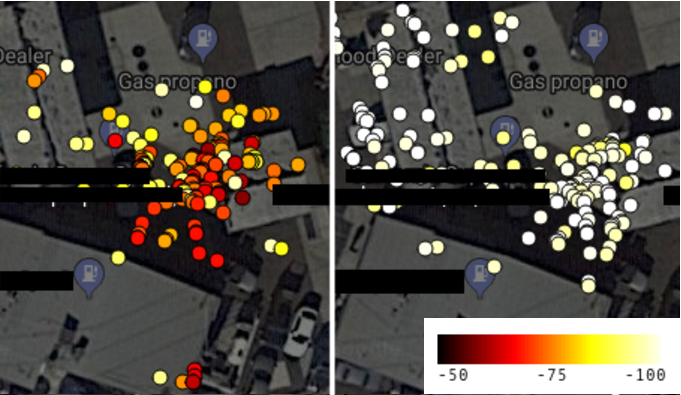
\includegraphics[width=\linewidth]{fig/rssi_motivation.pdf}
\caption{
\label{fig:rssi}
  Combining RSSI data with satellite imagery reveals if a device is located in the pump area of a gas station.
}
\end{figure}

When the skimmer responds to the Bluetooth scan request it responds with a
packet that contains the device's MAC address and class of device, and the
scanner uses the signal strength of this received packet to measure RSSI.
%
By the nature of being installed inside a gas pump, which is often a metal box,
the Bluetooth signal strength is typically only strong in the pump area.
%
Other devices that we suspected may be skimmers, all had a low signal strength
in the pump area, because aside from the cars parked at the pumps, the only
places where a Bluetooth device would be located in the pump area would be
inside the pump.
%
We show this by combining the RSSI with the geo-location from GPS, and satellite
imagery of the gas station, it becomes clear that the inside of a gas pump
(example shown in Figure~\ref{fig:rssi}).
%
While at a gas station this can be seen by moving toward the pump area to see
if the device's signal strength increases. 



\fi %}}}
